\hypertarget{day-10---ux7528ux6237ux6ce8ux518cux548cux767bux5f55}{%
\subsection{Day 10 -
用户注册和登录}\label{day-10---ux7528ux6237ux6ce8ux518cux548cux767bux5f55}}

用户管理是绝大部分 Web
网站都需要解决的问题。用户管理涉及到用户注册和登录。

用户注册相对简单,我们可以先通过 API 把用户注册这个功能实现了:

\begin{pythoncode}
_RE_EMAIL = re.compile(r'^[a-z0-9\.\-\_]+\@[a-z0-9\-\_]+(\.[a-z0-9\-\_]+){1,4}$')
_RE_SHA1 = re.compile(r'^[0-9a-f]{40}$')

@post('/api/users')
def api_register_user(*, email, name, passwd):
    if not name or not name.strip():
        raise APIValueError('name')
    if not email or not _RE_EMAIL.match(email):
        raise APIValueError('email')
    if not passwd or not _RE_SHA1.match(passwd):
        raise APIValueError('passwd')
    users = yield from User.findAll('email=?', [email])
    if len(users) > 0:
        raise APIError('register:failed', 'email', 'Email is already in use.')
    uid = next_id()
    sha1_passwd = '%s:%s' % (uid, passwd)
    user = User(id=uid, name=name.strip(), email=email, passwd=hashlib.sha1(sha1_passwd.encode('utf-8')).hexdigest(), image='http://www.gravatar.com/avatar/%s?d=mm&s=120' % hashlib.md5(email.encode('utf-8')).hexdigest())
    yield from user.save()
    
    r = web.Response()
    r.set_cookie(COOKIE_NAME, user2cookie(user, 86400), max_age=86400, httponly=True)
    user.passwd = '******'
    r.content_type = 'application/json'
    r.body = json.dumps(user, ensure_ascii=False).encode('utf-8')
    return r
\end{pythoncode}

注意用户口令是客户端传递的经过 SHA1 计算后的 40 位 Hash
字符串,所以服务器端并不知道用户的原始口令。

接下来可以创建一个注册页面,让用户填写注册表单,然后,提交数据到注册用户的
API:

\begin{pythoncode}


注册



<script>
function validateEmail(email) {
    var re = /^[a-z0-9\.\-\_]+\@[a-z0-9\-\_]+(\.[a-z0-9\-\_]+){1,4}$/;
    return re.test(email.toLowerCase());
}
$(function () {
    var vm = new Vue({
        el: '#vm',
        data: {
            name: '',
            email: '',
            password1: '',
            password2: ''
        },
        methods: {
            submit: function (event) {
                event.preventDefault();
                var $form = $('#vm');
                if (! this.name.trim()) {
                    return $form.showFormError('请输入名字');
                }
                if (! validateEmail(this.email.trim().toLowerCase())) {
                    return $form.showFormError('请输入正确的Email地址');
                }
                if (this.password1.length < 6) {
                    return $form.showFormError('口令长度至少为6个字符');
                }
                if (this.password1 !== this.password2) {
                    return $form.showFormError('两次输入的口令不一致');
                }
                var email = this.email.trim().toLowerCase();
                $form.postJSON('/api/users', {
                    name: this.name.trim(),
                    email: email,
                    passwd: CryptoJS.SHA1(email + ':' + this.password1).toString()
                }, function (err, r) {
                    if (err) {
                        return $form.showFormError(err);
                    }
                    return location.assign('/');
                });
            }
        }
    });
    $('#vm').show();
});
</script>





    <div class="uk-width-2-3">
        <h1>欢迎注册!</h1>
        <form id="vm" v-on="submit: submit" class="uk-form uk-form-stacked">
            <div class="uk-alert uk-alert-danger uk-hidden"></div>
            <div class="uk-form-row">
                <label class="uk-form-label">名字:</label>
                <div class="uk-form-controls">
                    <input v-model="name" type="text" maxlength="50" placeholder="名字" class="uk-width-1-1">
                </div>
            </div>
            <div class="uk-form-row">
                <label class="uk-form-label">电子邮件:</label>
                <div class="uk-form-controls">
                    <input v-model="email" type="text" maxlength="50" placeholder="your-name@example.com" class="uk-width-1-1">
                </div>
            </div>
            <div class="uk-form-row">
                <label class="uk-form-label">输入口令:</label>
                <div class="uk-form-controls">
                    <input v-model="password1" type="password" maxlength="50" placeholder="输入口令" class="uk-width-1-1">
                </div>
            </div>
            <div class="uk-form-row">
                <label class="uk-form-label">重复口令:</label>
                <div class="uk-form-controls">
                    <input v-model="password2" type="password" maxlength="50" placeholder="重复口令" class="uk-width-1-1">
                </div>
            </div>
            <div class="uk-form-row">
                <button type="submit" class="uk-button uk-button-primary"><i class="uk-icon-user"></i> 注册</button>
            </div>
        </form>
    </div>


\end{pythoncode}

这样我们就把用户注册的功能完成了:

 
 \begin{figure}[htp]
	\centering
	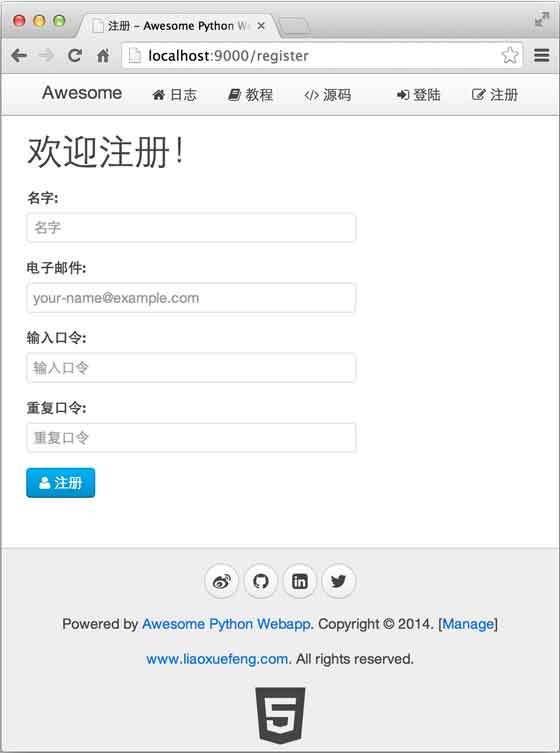
\includegraphics[width=0.6\linewidth]{fig/955719702776576.png}
\end{figure}


用户登录比用户注册复杂。由于 HTTP
协议是一种无状态协议,而服务器要跟踪用户状态,就只能通过 cookie
实现。大多数 Web 框架提供了 Session 功能来封装保存用户状态的 cookie。

Session 的优点是简单易用,可以直接从 Session 中取出用户登录信息。

Session
的缺点是服务器需要在内存中维护一个映射表来存储用户登录信息,如果有两台以上服务器,就需要对
Session 做集群,因此,使用 Session 的 Web App 很难扩展。

我们采用直接读取 cookie 的方式来验证用户登录,每次用户访问任意
URL,都会对 cookie 进行验证,这种方式的好处是保证服务器处理任意的 URL
都是无状态的,可以扩展到多台服务器。

由于登录成功后是由服务器生成一个 cookie 发送给浏览器,所以,要保证这个
cookie 不会被客户端伪造出来。

实现防伪造 cookie 的关键是通过一个单向算法(例如 SHA1),举例如下:

当用户输入了正确的口令登录成功后,服务器可以从数据库取到用户的
id,并按照如下方式计算出一个字符串:

\begin{pythoncode}
"用户id" + "过期时间" + SHA1("用户id" + "用户口令" + "过期时间" + "SecretKey")
\end{pythoncode}

当浏览器发送 cookie 到服务器端后,服务器可以拿到的信息包括:

\begin{itemize}
\item
  用户 id
\item
  过期时间
\item
  SHA1 值
\end{itemize}

如果未到过期时间,服务器就根据用户 id 查找用户口令,并计算:

\begin{pythoncode}
SHA1("用户id" + "用户口令" + "过期时间" + "SecretKey")
\end{pythoncode}

并与浏览器 cookie
中的哈希进行比较,如果相等,则说明用户已登录,否则,cookie 就是伪造的。

这个算法的关键在于 SHA1 是一种单向算法,即可以通过原始字符串计算出 SHA1
结果,但无法通过 SHA1 结果反推出原始字符串。

所以登录 API 可以实现如下:

\begin{pythoncode}
@post('/api/authenticate')
def authenticate(*, email, passwd):
    if not email:
        raise APIValueError('email', 'Invalid email.')
    if not passwd:
        raise APIValueError('passwd', 'Invalid password.')
    users = yield from User.findAll('email=?', [email])
    if len(users) == 0:
        raise APIValueError('email', 'Email not exist.')
    user = users[0]
    
    sha1 = hashlib.sha1()
    sha1.update(user.id.encode('utf-8'))
    sha1.update(b':')
    sha1.update(passwd.encode('utf-8'))
    if user.passwd != sha1.hexdigest():
        raise APIValueError('passwd', 'Invalid password.')
    
    r = web.Response()
    r.set_cookie(COOKIE_NAME, user2cookie(user, 86400), max_age=86400, httponly=True)
    user.passwd = '******'
    r.content_type = 'application/json'
    r.body = json.dumps(user, ensure_ascii=False).encode('utf-8')
    return r
    

def user2cookie(user, max_age):
    
    expires = str(int(time.time() + max_age))
    s = '%s-%s-%s-%s' % (user.id, user.passwd, expires, _COOKIE_KEY)
    L = [user.id, expires, hashlib.sha1(s.encode('utf-8')).hexdigest()]
    return '-'.join(L)
\end{pythoncode}

对于每个 URL 处理函数,如果我们都去写解析 cookie
的代码,那会导致代码重复很多次。

利用 middle 在处理 URL 之前,把 cookie
解析出来,并将登录用户绑定到\texttt{request}对象上,这样,后续的 URL
处理函数就可以直接拿到登录用户:

\begin{pythoncode}
@asyncio.coroutine
def auth_factory(app, handler):
    @asyncio.coroutine
    def auth(request):
        logging.info('check user: %s %s' % (request.method, request.path))
        request.__user__ = None
        cookie_str = request.cookies.get(COOKIE_NAME)
        if cookie_str:
            user = yield from cookie2user(cookie_str)
            if user:
                logging.info('set current user: %s' % user.email)
                request.__user__ = user
        return (yield from handler(request))
    return auth
    

@asyncio.coroutine
def cookie2user(cookie_str):
    '''
    Parse cookie and load user if cookie is valid.
    '''
    if not cookie_str:
        return None
    try:
        L = cookie_str.split('-')
        if len(L) != 3:
            return None
        uid, expires, sha1 = L
        if int(expires) < time.time():
            return None
        user = yield from User.find(uid)
        if user is None:
            return None
        s = '%s-%s-%s-%s' % (uid, user.passwd, expires, _COOKIE_KEY)
        if sha1 != hashlib.sha1(s.encode('utf-8')).hexdigest():
            logging.info('invalid sha1')
            return None
        user.passwd = '******'
        return user
    except Exception as e:
        logging.exception(e)
        return None
\end{pythoncode}

这样,我们就完成了用户注册和登录的功能。

\hypertarget{ux53c2ux8003ux6e90ux7801}{%
\subsubsection{参考源码}\label{ux53c2ux8003ux6e90ux7801}}

\href{https://github.com/michaelliao/awesome-python3-webapp/tree/day-10}{day-10}

